\documentclass[tikz]{standalone}
\usepackage{tikz} 
\usetikzlibrary{shapes.misc,patterns,hobby}
\usepackage{pgfplots}
\usepgfplotslibrary{fillbetween}
%\usepackage[active,tightpage]{preview}  %generates a tightly fitting border around the work
%\PreviewEnvironment{tikzpicture}
%\setlength\PreviewBorder{2mm}
\usepackage{xcolor}
\definecolor{myred}{RGB}{196,19,47} 
\definecolor{myblue}{RGB}{0,139,139}

\begin{document}
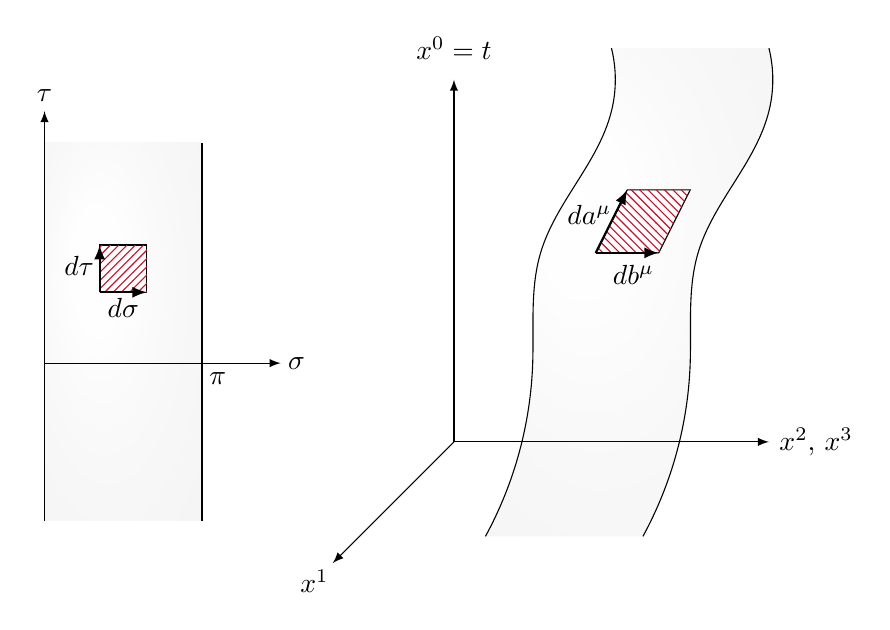
\begin{tikzpicture}[xscale=2,yscale=2,>=latex]
%Koordinatensystem links mit Beschriftung 
\shade[ball color = gray!30, opacity = 0.05] plot coordinates {(0.4,-1) (1.4,-1) (1.4,1.4) (0.4,1.4)}; 

\draw[->, thin] (0.4,-1) to (0.4,1.6);
\node at (0.4,1.7) {$\tau$};
\draw[->, thin] (0.4,0) to (1.9,0);
\node at (2,0) {$\sigma$};
\draw[-, thin] (1.4,-1) to (1.4,1.4);
\node at (1.5,-0.1) {$\pi$};

%Quadrat unten
\path[draw, color = black, thin] (0.75,0.45) to (1.05,0.45) to (1.05,0.75) to (0.75,0.75) to (0.75,0.45);
\path[pattern=north east lines, pattern color=myred] plot coordinates {(0.75,0.45) (1.05,0.45) (1.05,0.75) (0.75,0.75)};
\draw[->, thick] (0.75,0.45) to (1.05,0.45);
\node at (0.9,0.35) {$d\sigma$};
\draw[->, thick] (0.75,0.45) to (0.75,0.75);
\node at (0.62,0.62) {$d\tau$};


%Koordinatensystem rechts (3D)
\draw[->, thin] (3,-0.5,0) to (3,-0.5,2);
\node at (3,-0.5,2.3) {$x^1$};
\draw[->, thin] (3,-0.5,0) to (5,-0.5,0);
\node at (5.3,-0.5,0) {$x^2$, $x^3$};
\draw[->, thin] (3,-0.5,0) to (3,1.8,0);
\node at (3,2,0) {$x^0 = t$};

%Parallele Linien rechts in der Mitte
\newcommand\kurve{(3.2,-1.1) to [curve through = { (3.5,0) (3.55,0.7) (4,1.6)  }] (4,2)}
\newcommand\kurvee{(5,2) to [curve through = { (5,1.6) (4.55,0.7) (4.5,0) }] (4.2,-1.1)}

\def\mypath{\kurve -- \kurvee -- (3.2,-1.1)}

\draw[-] \kurve;
\draw[-] \kurvee;

\shade[ball color = gray!30, opacity = 0.05] \mypath;
\path[draw, color = black, thin] (3.9,0.7) to (4.3,0.7) to (4.5,1.1) to (4.1,1.1) to (3.9,0.7);
\path[pattern=north west lines, pattern color=myred] plot coordinates {(3.9,0.7) (4.3,0.7) (4.5,1.1) (4.1,1.1)};
\node at (3.86,0.94) {$da^{\mu}$};
\draw[->, thick] (3.9,0.7) to (4.1,1.1);
\node at (4.14,0.56) {$db^{\mu}$};
\draw[->, thick] (3.9,0.7) to (4.3,0.7);

\end{tikzpicture}
\end{document}
